% !TeX TXS-program:compile = txs:///pdflatex/[--shell-escape]
\documentclass[10pt,landscape,a4paper]{article}
\usepackage[table]{xcolor}
\usepackage[normalem]{ulem}
\usepackage{tikz}
\usetikzlibrary{shapes,positioning,arrows,fit,calc,graphs,graphs.standard}
\usepackage[nosf]{kpfonts}
\usepackage[t1]{sourcesanspro}
\usepackage{multicol}
\usepackage{wrapfig}
\usepackage[top=1mm,bottom=1mm,left=1mm,right=1mm]{geometry}
\usepackage[framemethod=tikz]{mdframed}
\usepackage{microtype}
\usepackage{tabularx}
\usepackage{hhline}
\usepackage{makecell}
\usepackage{mathtools}
\usepackage{subfig}
\usepackage{listings}
\usepackage{soul}
\usepackage{amsmath,amsthm,amsfonts,amssymb}
\usepackage{adjustbox}

\graphicspath{ {./img/} }

\DeclarePairedDelimiter{\ceil}{\lceil}{\rceil}

\definecolor{myblue}{cmyk}{1,.72,0,.38}

\pgfdeclarelayer{background}
\pgfsetlayers{background,main}

\renewcommand{\baselinestretch}{.8}
\pagestyle{empty}

\let\counterwithout\relax
\let\counterwithin\relax
\usepackage{chngcntr}
\usepackage{verbatim}
\usepackage{etoolbox}
\makeatletter
\preto{\@verbatim}{\topsep=0pt \partopsep=0pt }
\makeatother

\counterwithin*{equation}{section}
\counterwithin*{equation}{subsection}
\usepackage{enumitem}
\newlist{legal}{enumerate}{10}
\setlist[legal]{label*=\arabic*.,leftmargin=3mm}
\setlist[itemize]{leftmargin=3mm}
\setlist[enumerate]{leftmargin=3.5mm}
\setlist{nosep}
\usepackage{minted}

\newenvironment{conditions*}
{\par\vspace{\abovedisplayskip}\noindent
	\tabularx{\columnwidth}{>{$}l<{$} @{\ : } >{\raggedright\arraybackslash}X}}
{\endtabularx\par\vspace{\belowdisplayskip}}
\newenvironment{descitemize} % a mixture of description and itemize
{\begin{description}[leftmargin=*,before=\let\makelabel\descitemlabel]}
	{\end{description}}
\newcommand{\descitemlabel}[1]{%
	\textbullet\ \textbf{#1}%
}
\makeatletter

\renewcommand{\section}{\@startsection{section}{1}{0mm}%
	{.2ex}%
	{.2ex}%x
	{\color{myblue}\sffamily\small\bfseries}}
\renewcommand{\subsection}{\@startsection{subsection}{1}{0mm}%
	{.2ex}%
	{.2ex}%x
	{\sffamily\bfseries}}
\renewcommand{\subsubsection}{\@startsection{subsubsection}{1}{0mm}%
	{.2ex}%
	{.2ex}%x
	{\rmfamily\bfseries}}

\makeatother
\setlength{\parindent}{0pt}
\setminted{tabsize=2, breaklines}
% Remove belowskip of minted
\setlength\partopsep{-\topsep}

\newcolumntype{a}{>{\hsize=1.5\hsize}X}
\newcolumntype{b}{>{\hsize=.25\hsize}X}

\setlength\columnsep{10pt}
\setlength\columnseprule{0pt}
\begin{document}
	\abovedisplayskip=0pt
	\abovedisplayshortskip=0pt
	\belowdisplayskip=0pt
	\belowdisplayshortskip=0pt
%	\scriptsize
	\tiny
	\begin{multicols*}{4}
		\section{Intro to OTM}
		\subsection{What is Operations}
		\begin{itemize}
			\item Part of business organization that is responsible for producing (tangible) goods and services
			\item It is a \textcolor{red}{business function} responsible for designing, managing and improving creation and delivery of products
		\end{itemize}
		\subsubsection{Products vs Services}
		\begin{center}
			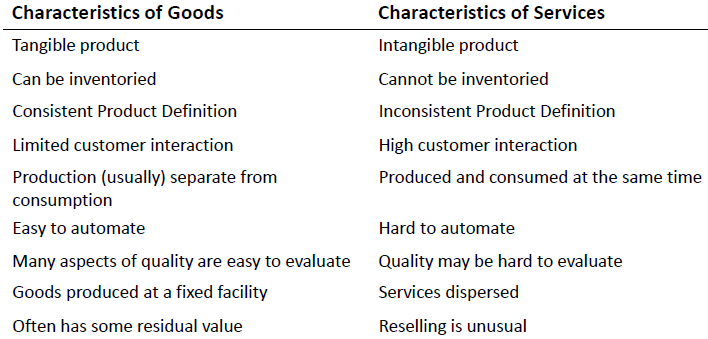
\includegraphics[width=0.6\columnwidth]{goods_vs_service}
		\end{center}
		\begin{itemize}
			%			\item Products are physical items that include raw materials, parts, subassemblies, and final products
			%			\item Services are activities that provide some combination of time, location, form or psychological value
			\item In most cases, products are a mix of both physical goods and service
		\end{itemize}
		\subsubsection{Supply Chain}
		\begin{itemize}
			\item Network of all entities involved in producing and delivering finished product to customer.
		\end{itemize}
		\begin{center}
			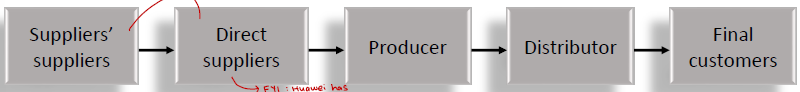
\includegraphics[width=0.7\columnwidth]{supply_chain}
		\end{center}
		\begin{itemize}
			\item Supply chain management integrates supply
			and demand management within and across companies. Without it companies faces:
			\begin{itemize}
				\item Oscillating inventory levels (bullwhip effect $\rightarrow$ surge in retail causes large change in inventory down supply chain), inventory stockouts, late deliveries and quality problems
			\end{itemize}
		\end{itemize}
		\subsection{Functions of Business Organization}
		\begin{itemize}
			\item \textbf{Marketing} (generates demand), \textbf{Operations} (create product/service), \textbf{Finance} (deals with money)
			\item Function overlaps:
			\begin{itemize}
				\item Finance and Ops: budget, analysis of investments, provision of funds
				\item Marketing and Ops: Demand data, product designs, competitor analysis, lead time data
			\end{itemize}
		\end{itemize}
		\subsection{Objectives of Ops Management}
		\begin{itemize}
			\item \textbf{Cost} (productivity, inventory turnover), \textbf{Quality} (features, mean time between failures, scraps), \textbf{Dependability} (\% of on-time deliveries, days late), \textbf{Flexibility} (setup times, time to market)
		\end{itemize}
		\subsubsection{Decisions in Ops Planning}
		\begin{center}
			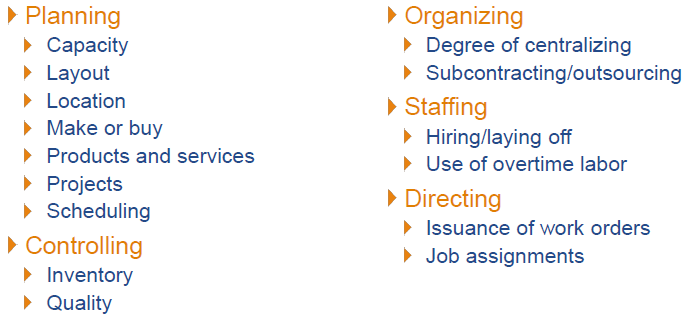
\includegraphics[width=0.6\columnwidth]{decisions_in_ops}
		\end{center}
		\subsection{Productivity Calculations}
		$$\text{Productivity}=\dfrac{\text{Output}}{\text{Input}}$$
		$$\text{\% change in productivity}=\dfrac{\text{1+Y\%}}{\text{1+X\%}}-1$$
		$$\text{Multifactor Productivity}=\dfrac{\text{Output}}{\text{Labor + Material + Energy + Capital + Misc}}$$
		$$\text{Relative Wage Rates}=\dfrac{\text{Foreign Wage Rate}}{\text{Exchange Rate}} \times \dfrac{\text{Home Productivity}}{\text{Foreign Productivity}}$$
		\begin{itemize}
			\item How to increase productivity in Services due to it being labor intensive, requires domain specific skills, difficult to automate
		\end{itemize}
		\section{Operation Processes and Technologies}
		\subsection{Process Selection}
		\begin{itemize}
			\item refers to the way production of goods/services will be organized which impacts: capacity planning, layout of facilities, equipment and design of work systems
		\end{itemize}
		\subsection{Types of Processes}
%		\begin{enumerate}
%			\item \textbf{Job Shop} - low volume, high variety (e.g. Salon shop, clinics)
%			\begin{itemize}
%				\item highly customized goods, process focused, processing is intermittent and work using general-purpose equipment and skilled workers
%				\item Faces challenge in assigning workers to activities (sequencing)
%				\item Uses analytical tools in optimization with heuristics like trial and error and rule of thumb
%				\item Trade off of Flexibility vs Cost (idle time, labor skills, inventory)
%			\end{itemize}
%			\item \textbf{Batch} - Mid volume, mid variety (e.g. Bakery, movie theaters)
%			\begin{itemize}
%				\item Production of identical products made in batches
%				\item Equipment used need not be as flexible but processing still intermittent
%				\item Skill level does not need to be as high due to lesser variety
%				\item Faces challenges in balance between variety and volume and reducing setup times
%				\item Trade off between Variety and Cost (batch size affect EoS and inventory)
%			\end{itemize}
%			\item \textbf{Repetitive} - High volume, low variety (e.g. Car parts production, cafeteria lines, ticket collectors)
%			\begin{itemize}
%				\item Only slight flexibility of equipment, skills of workers are low, can be worker/machine paced
%				\item Faces challenge in activity design - aim to balance line and optimize cycle times
%				\item Trade off of Speed vs Cost (inventory)
%			\end{itemize}
%			\item \textbf{Continuous} - Very high volume, very little variety (e.g. Oil refinery)
%			\begin{itemize}
%				\item Product focused, no need for equipment flexibility, skills can range from low to high depending on complexity of system
%				\item Faces challenge in ensuring continuous maintenance and supply (shift work)
%			\end{itemize}
%			\item \textbf{Project} - Non-routine, one of a kind (e.g. Building a bridge, making a movie
%			\begin{itemize}
%				\item Faces challenges in achieve project goals within time frame, solved using Critical Path Method/Program Evaluation Review Technique
%			\end{itemize}
%		\end{enumerate}
		\begin{center}
			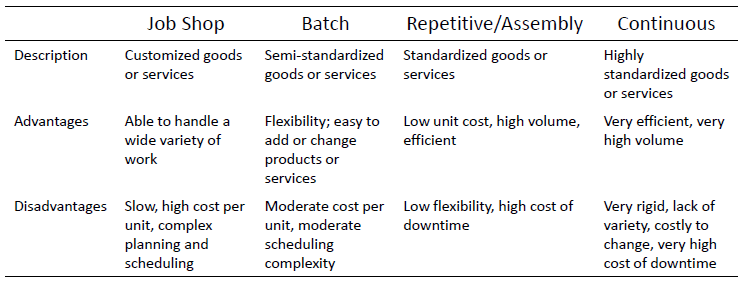
\includegraphics[width=0.7\columnwidth]{processing_types}
		\end{center}
		\subsubsection{Process and Products Layouts}
		\begin{center}
			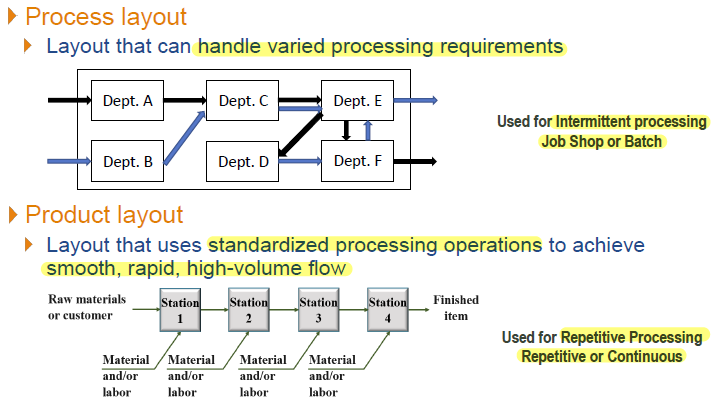
\includegraphics[width=0.6\columnwidth]{process_layouts}
		\end{center}
		\subsubsection{Summary}
		\begin{center}
			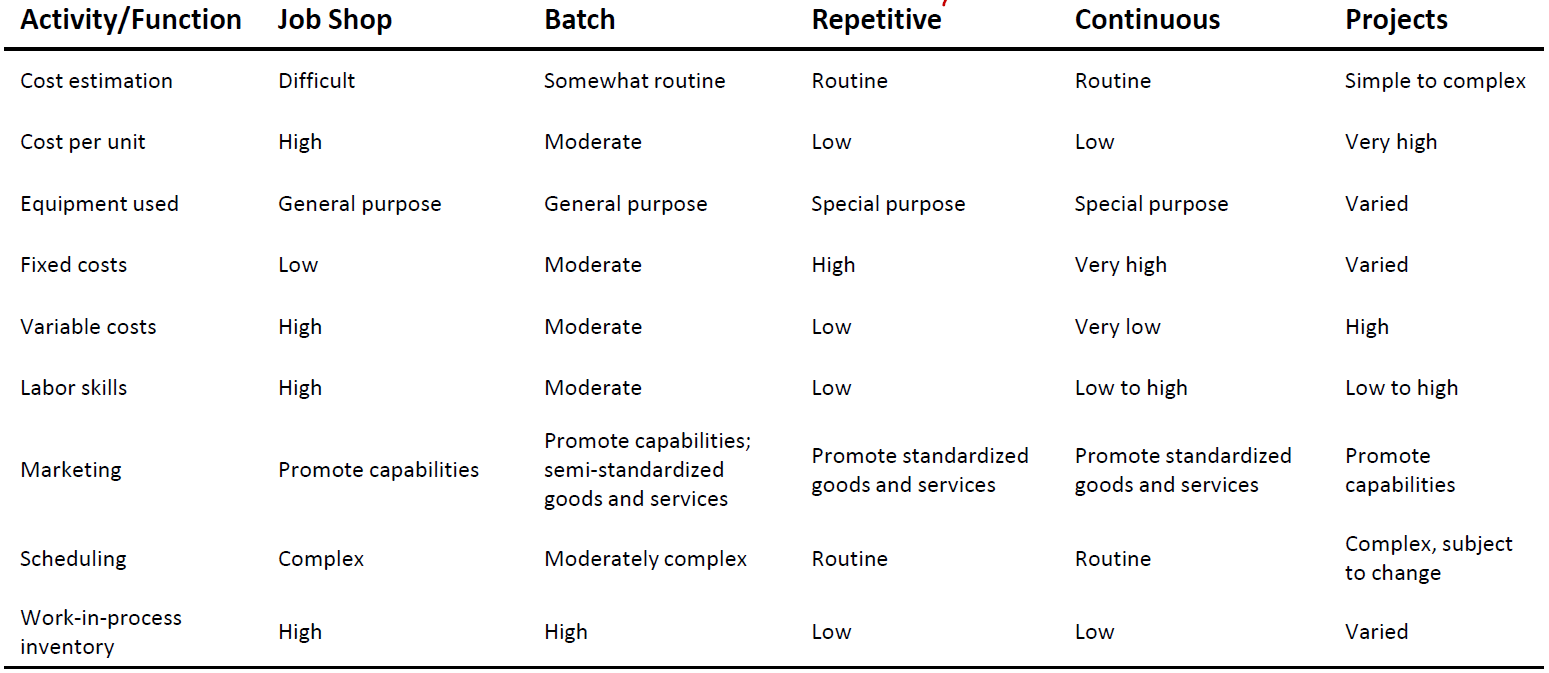
\includegraphics[width=0.6\columnwidth]{process_summary}
		\end{center}
		\subsection{Technology}
		\begin{itemize}
			\item Technology refers to application of scientific knowledge to development and improvement of goods and services
			\begin{itemize}
				\item \textbf{Hard Technologies} are equipment or deceives like actuators, computers and sensors
				\item \textbf{Soft Technologies} are application of the internet, software and information system like databases, AI, and voice recognition software
			\end{itemize}
			\item 3 types of Automation:
			\begin{itemize}
				\item \textbf{Fixed automation}: use high cost specialized equipment for fixed sequence of ops, suitable to produce large volumes of goods but minimal variety (e.g. automated car park system, machining transfer lines in automobile)
				\item \textbf{Programmable automation}: use general-purpose equipment controlled by a program, suitable for batch operations where for each batch, the equipment has to be reprogrammed. Production rates lower than fixed automation (e.g. CAD and CAE)
				\item \textbf{Flexible Automation}: use equipment more customized that that of programmable automation, suitable when variety is sufficiently limited. Reprogramming typically done off-line and allows for mixture of different products to be produced one after another.
			\end{itemize}
		\end{itemize}
		\section{Process Flows}
		\subsection{Process Analysis}
		\begin{itemize}
			\item \textbf{Flow unit}: basic unit of analysis
			\item \textbf{Activity/Process Time}: amount of time spend on activity, including setup and run time
			\item \textbf{Process Capacity}: maximum number of flow units that move through the process 
			\item \textbf{Inventory}: average number of flow units that are in the process
			\item \textbf{Buffer}: storage area between stages where the output of a stage is placed prior to being used in a downstream stage. Should contain enough units to prevent starvation and used to improve throughput
			\item \textbf{Little's Law}: Inventory = Flow Rate $\times$ Flow Time
			\item \textbf{Number of stages required}: Total activity time / Cycle Time
		\end{itemize}
		\begin{tabular}{c c}
			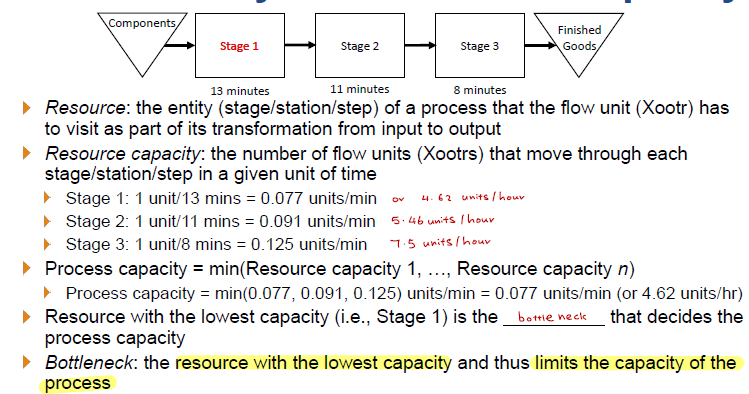
\includegraphics[width=0.5\linewidth]{process_analysis_terms}
			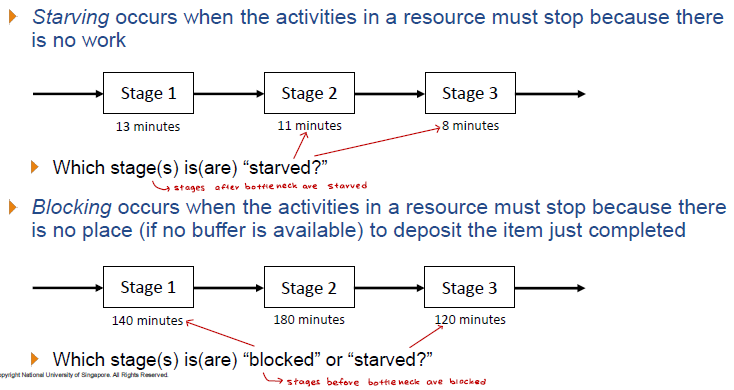
\includegraphics[width=0.5\linewidth]{bottlenecks}
		\end{tabular}
		\begin{tabular}{c c}
			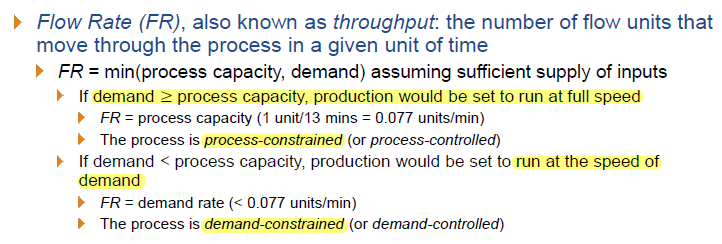
\includegraphics[width=0.5\linewidth]{flow_rate}
			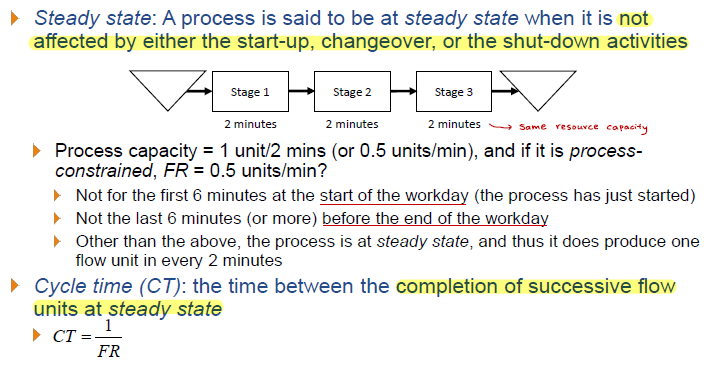
\includegraphics[width=0.5\linewidth]{cycle_time}
		\end{tabular}
		\begin{tabular}{c c}
			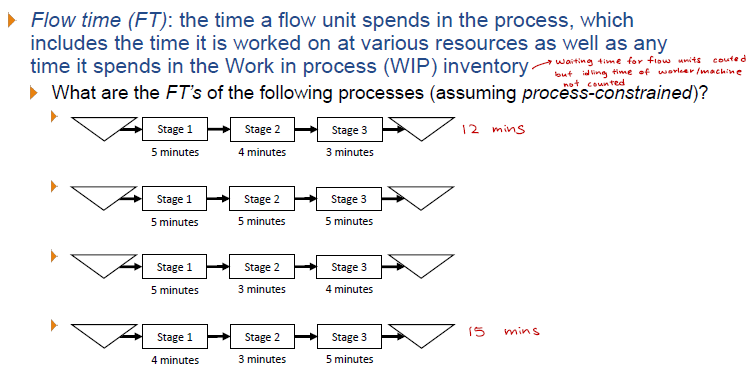
\includegraphics[width=0.5\linewidth]{flow_time}
			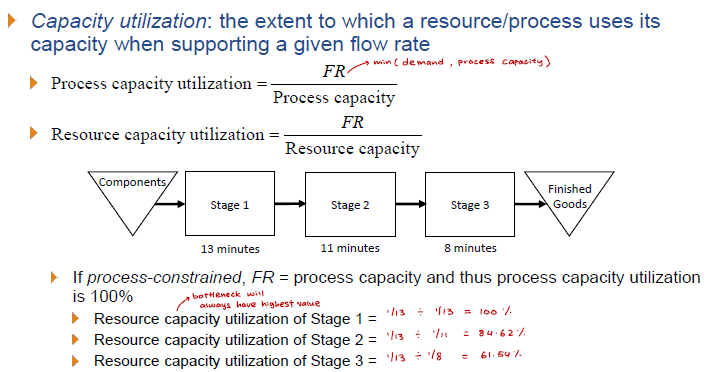
\includegraphics[width=0.5\linewidth]{capacity_utilization}
		\end{tabular}
		\begin{tabular}{c c}
			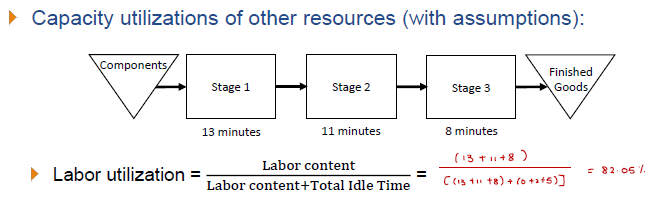
\includegraphics[width=0.5\linewidth]{labor_utilization}
			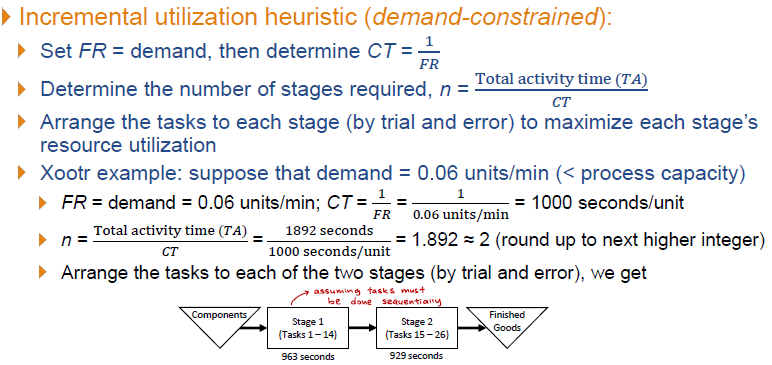
\includegraphics[width=0.5\linewidth]{line_balancing1}
		\end{tabular}
		\begin{tabular}{c c}
			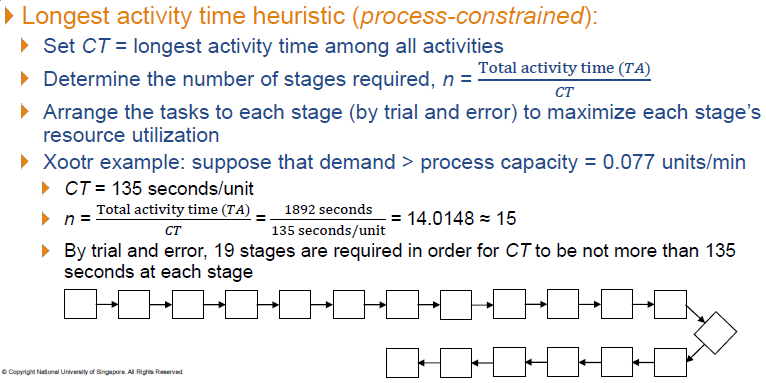
\includegraphics[width=0.5\linewidth]{line_balancing2}
			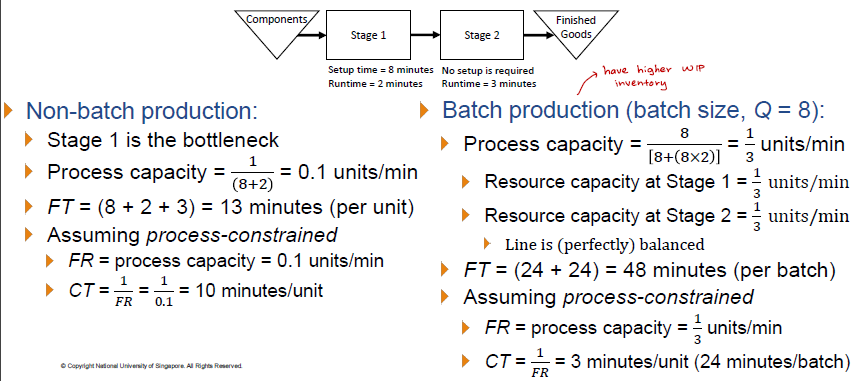
\includegraphics[width=0.5\linewidth]{batch_produce}
		\end{tabular}
		\section{Aggregate Planning}
		\subsection{Planning Horizons}
		\begin{itemize}
			\item Aggregate planning: Intermediate-range capacity planning, usually covering at least \textbf{one seasonal cycle (2 to 12 months)}
			\item \textbf{Long-range planning}: > 1 year, yearly increments. Planning for things like Long-term capacity; location; layout; product design; work system design
			\item \textbf{Intermediate- range planning}: 1 seasonal cycle, monthly or quarterly increments. Planning for things like: Employment; output; finished-goods inventories; subcontracting; backorders
			\item \textbf{Short-range planning} (reliable planning): 1 day to < 6 months, weekly increments. Planning for things like: Production lot size; order quantities; machine loading; job assignments/sequencing; work schedules
		\end{itemize}
		\begin{center}
			\includegraphics[width=0.45\columnwidth]{planning_horizon}
		\end{center}
		\subsection{Aggregate Production Planning}
		Aims to specify the \textbf{production rate} (units produced), \textbf{employment level} (\# of workers), \textbf{inventory on hand} (carried from previous period), in order to meet the varying demand patter over seasonal cycle. Ultimately want to \textbf{reduce cost}, \textbf{maintain service level} and \textbf{minimize workforce fluctuations}
		\subsubsection{Inputs and Outputs}
		\begin{tabular}{c c}
			\adjustbox{valign=T}{\includegraphics[width=0.45\linewidth]{agg_plan_input}}
			\adjustbox{valign=T}{\includegraphics[width=0.45\linewidth]{agg_plan_output}}
		\end{tabular}
		\subsubsection{Strategies}
		\begin{itemize}
			\item Demand Management
			\begin{itemize}
				\item Influence demand through promotion (however there will be a lag between promotion and demand); pricing; backorders
				\item Create new demand for complementary products
			\end{itemize}
			\item Supply management
			\begin{itemize}
				\item Level capacity strategy
				\begin{itemize}
					\item Maintain a level workforce/steady output rate
					\item Use inventory/backorders to absorb variations in demand
					\item Works best when inventory-carrying and backlog costs are relatively low
				\end{itemize}
				\item Chase demand strategy
				\begin{itemize}
					\item Match demand period by period; hire/fire; OT/Slack time; part-timers; subcon
					\item Works best when inventory-carrying costs are high, and costs of changing capacity are low
				\end{itemize}
			\end{itemize}
		\end{itemize}
		\begin{tabular}{c c}
			\includegraphics[width=0.6\linewidth]{agg_plan_strat}
			\includegraphics[width=0.4\linewidth]{agg_plan_techniques}
		\end{tabular}
		\begin{tabular}{c c}
			\includegraphics[width=0.5\linewidth]{level_cap}
			\includegraphics[width=0.5\linewidth]{chase_demand}
		\end{tabular}
		\subsubsection{Aggregate Planning in Services}
		Difficulties faced when doing aggregate planning for services:
		\begin{itemize}
			\item Services occur when they are rendered - cannot be inventoried
			\item Demand for services highly variable and unpredictable
			\item Capacity availability hard to predict - labor intensive and service task requirements highly variable
		\end{itemize}
		\subsection{Master Schedule}
		Result of \textbf{disaggregating} an aggregate plan - shows quantity and timing of specific end items for a schedule horizon
		\begin{itemize}
			\item Master Production Schedule
			\begin{itemize}
				\item Indicates the quantity and timing of planned production, taking into account desired delivery quantity and timing as well as on-hand inventory
			\end{itemize}
			\item Production Planning and Control (PP\&C)
			\begin{itemize}
				\item Determines the quantities needed to meet demand
				\item Interfaces with marketing, capacity, production, and distribution plannings
				\item Enables the senior management to determine whether the business plan and its strategic objectives will be achieved
			\end{itemize}
			\item Used as \textbf{input for Material Requirements Planning}
		\end{itemize}
		\begin{center}
			\includegraphics[width=0.65\columnwidth]{master_schedule}
		\end{center}
		\subsubsection{Master Schedule Examples}
		\begin{tabular}{c c}
			\includegraphics[width=0.5\linewidth]{ms_ex_1}
			\includegraphics[width=0.5\linewidth]{ms_ex_2}
		\end{tabular}
		\subsubsection{Time Fences}
		\begin{itemize}
			\item \textbf{Frozen phase}: near-term phase (1-3 periods) that is so soon that delivery of a new order would be impossible, or only possible using very costly or extraordinary options such as delaying another delivery (no adjustment to master schedule)
			\item \textbf{Slushy phase}: next phase, and its time fence is usually a few periods beyond the frozen phase (4-5 periods). Order entry in this phase necessitate trade-offs, but is less costly or disruptive than in frozen phase
			\item \textbf{Liquid phase}: farthest out on the time horizon (>=6 periods). New orders or cancellations can be entered with ease 
		\end{itemize}
		\section{Inventory Management}
		\subsection{Major Objectives of Companies}
		\begin{itemize}
			\item Maximise customer service level
			\item efficient low-cost operations
			\item minimize investment in inventory
		\end{itemize}
		\subsection{What is inventory?}
		\begin{itemize}
			\item Raw materials and purchased parts
			\item Partially completed goods, called work-in-process (WIP)
			\item Finished-goods inventories (manufacturing firms) or merchandise (retail stores)
			\item Maintenance, repairs, and operations (MRO) inventory (e.g. drill bits, cleaning products)
			\item Goods-in-transit to warehouses, distributors, or customers (pipeline inventory)
		\end{itemize}
		\subsubsection{Functions/Purpose of Inventory}
		\begin{itemize}
			\item Manage \textbf{Production}: permit ops (pipeline stock), smooth production requirements (seasonal stock), decouple ops (buffer stock)
			\item Manage \textbf{Demand}: meet anticipated demand, protect against shortages (safety stock)
			\item \textbf{Control costs}: take advantage of order/production cycles, hedge against inflation, take advantage of quantity discounts (economic of scale)
		\end{itemize}
		\subsubsection{Cons of Inventory}
		\begin{itemize}
			\item Higher costs: ordering/setup costs and holding costs
			\item Difficult to control: determining optimal amount, record keeping, storage and maintenance (e.g. wine cellar)
			\item Handling inventory is a non-value-added activity
			\item Reduces cash availability
			\item Product might become obsolete
			\item Hides production problems (e.g. overprocessing, poor process capacity, breakdowns)
		\end{itemize}
		\subsection{ABC Analysis}
		Idea is to manage the 20\% of item that contributes to 80\% of the total inventory costs
		\begin{itemize}
			\item \textbf{Class A}: 15-20\% of total inventory items and represent 70-80\% of total dollar usage
			\begin{itemize}
				\item Intensive control, constant management attention, requires sophisticated forecasting
			\end{itemize}
			\item \textbf{Class B}: 30\% of total inventory items and represent
			15\%-25\% of the total dollar usage
			\begin{itemize}
				\item Moderate control using computer whenever possible
			\end{itemize}
			\item \textbf{Class C}: 50\%-55\% of total inventory items and
			represent 5\% of the total dollar usage
			\begin{itemize}
				\item Minimize control and transaction cost, use of simple manual control
			\end{itemize}
		\end{itemize}
		\subsection{Types of Inventories}
		\begin{itemize}
			\item \textbf{Dependent} (end product sold) vs \textbf{Independent} (component used in end product)
			\item \textbf{Deterministic} (demands known with certainty) vs. \textbf{Stochastic} (demands are uncertain)
			\item \textbf{Static} (Stationary) (expected demand does not change over time) vs. \textbf{Variable} (expected demand changes over time)
		\end{itemize}
		\subsection{Economic Order Quantity (EOQ)}
		\begin{itemize}
			\item Total Cost: Purchase + Ordering + Holding + Shortage cost
			\item To determine how much of a given item to order, we can use EOQ to get a good estimate
			\item Assumptions of EOQ model:
			\begin{itemize}
				\item Annual demand is known and is evenly spread throughout the year
				\item No stockouts are allowed
				\item Lead time is known and constant
				\item One-batch delivery (instant delivery)
				\item No quantity discount (\textbf{Purchase cost is ignored in EOQ})
				\item All other costs remain unchanged
				\item Order quantity can be a fraction
			\end{itemize}
			\item Average inventory levels are low when there are many orders, high if there are few orders
		\end{itemize}
		\begin{tabular}{c c}
			\includegraphics[width=0.5\linewidth]{eoq}
			\includegraphics[width=0.5\linewidth]{eoq_eg}
		\end{tabular}
		\begin{itemize}
			\item $Q^*=\sqrt{\dfrac{2DS}{H}}$,  $TIC^*=\sqrt{2DSH}$
			\item Ordering cost = holding cost when $Q = Q^*$
			\item Number of optimal order per period = $N^*=D/Q$
			\item Time between optimal order = $T^*=Q^*/D$ 
		\end{itemize}
		\subsection{Economic Production Quantity (EPQ)}
		\begin{itemize}
			\item Assumption is now that firms receive their inventories over a period of time instead of instantaneous delivery
			\item Suited for production environment where units are produced at a faster rate than they are used (sometimes also called Production Order Quantity (POQ)
			\item Lower (effective) holding cost than EOQ since avg inventory is lower
		\end{itemize}
		\begin{tabular}{c c}
			\includegraphics[width=0.5\linewidth]{epq_1}
			\includegraphics[width=0.5\linewidth]{epq_2}
		\end{tabular}
		\begin{tabular}{c c}
			\includegraphics[width=0.5\linewidth]{epq_eg}
			\includegraphics[width=0.5\linewidth]{discount_eg}
		\end{tabular}
		\begin{tabular}{c c}
			\includegraphics[width=0.5\linewidth]{discount_eg_2}
			\includegraphics[width=0.5\linewidth]{discount_eg_3}
		\end{tabular}
		\section{Inventory Management II}
		\subsection{Reorder Point Under Certainty}
		$$ ROP=d\times LT $$
		where
		\begin{conditions*}
			d & Demand rate (units per unit time) \\
			LT & Lead time (same units as $d$)
		\end{conditions*}
		\subsection{Fixed-Quantity Reorder Point}
		\begin{itemize}
			\item Safety stock: Difference between the maximum probable demand during lead time and expected demand during lead time
			\item ROP = Expected demand during lead time + Safety Stock
		\end{itemize}
		\subsubsection{How much safety stock?}
		\begin{itemize}
			\item Stockout risk: Risk of having a stockout that is determined by the ops manager, decreases when we increase stock which improves customer service level
			\item Service level: probability that demand will not exceed supply during lead time, calculated as 100\% - stockout risk
		\end{itemize}
		\begin{center}
			\includegraphics[width=0.5\columnwidth]{service-level}
		\end{center}
		\begin{itemize}
			\item Safety stock will depend on:
			\begin{itemize}
				\item Average demand rate and average lead time
				\item Demand and lead time variability
				\item Desired service level
			\end{itemize}
			\item Updated ROP equation:
		\end{itemize}
		\[\text{ROP = Expected demand during lead time + }z\sigma_{dLT}\]
		\begin{conditions*}
			z & Number of std dev (found in z table) \\
			\sigma_{dLT} & std dev of lead time demand
		\end{conditions*}
		\subsection{Only demand Uncertainty}
		\[\text{ROP}=\bar{d}\times LT+z\sigma_d\sqrt{LT}\]
		\begin{conditions*}
			\bar{d} & avg demand per period \\
			\sigma_d & std dev of demand per period
		\end{conditions*}
		\subsection{Only Lead Time Uncertainty}
		\[\text{ROP}=d\times\overline{LT}+zd\sigma_{LT}\]
		\begin{conditions*}
			d & Demand per period \\
			\sigma_{LT} & std dev of lead time \\
			\overline{LT} & Avg lead time
		\end{conditions*}
		\subsection{Both Demand and Lead Time Uncertainty}
		\[\text{ROP}=\bar{d}\times\overline{LT}+z\sqrt{\overline{LT}\sigma_d^2+\bar{d}^2\sigma_{LT}^2}\]
		\subsection{Fixed-Order-Interval Inventory Model}
		\begin{itemize}
			\item Orders are placed in fixed time intervals dictated by suppliers (consumers only vary order qty)
			\item Reasons for using FOI
			\begin{itemize}
				\item No need for continuous tracking of inventory (do inventory count just prior to placing order)
				\item Grouping orders from the same supplier yield savings in ordering/packing/transport costs
				\item Supplier’s policy may encourage its use
			\end{itemize}
		\end{itemize}
		\begin{center}
			\includegraphics[width=0.6\columnwidth]{FOI-model}
		\end{center}
		\[\text{ROP}=\bar{d}(OI+LT)+z\sigma_d\sqrt{OI+LT}-A\]
		\begin{conditions*}
			OI & Order interval (length of time between orders) \\ 
			A & Amount on hand at reorder time
		\end{conditions*}
		\section{Materials Requirements Planning (MRP)}
		\subsection{Inputs, Processing \& Outputs}
		\begin{itemize}
			\item MRP is a computer based system to order \& schedule \textcolor{red}{dependent demand} items
			\item Dependent demand items are items that are subassemblies; raw materials; component parts that are used in production of finished goods
		\end{itemize}
		\begin{center}
			\includegraphics[width=0.7\columnwidth]{mrp}
		\end{center}
		\begin{itemize}
			\item Bill of Materials/Product Structure Tree: List of materials, parts, subassemblies needed to produce end items
			\item Inventory Records: status of each item by time period (gross requirements, schedule receipts, expected amount on hand)
		\end{itemize}
		\begin{center}
			\includegraphics[width=0.65\columnwidth]{mrp-eg}
		\end{center}
		\subsection{Updating MRP}
		\begin{itemize}
			\item MRP is \textbf{not a static document} and have 2 approaches to deal with changes
			\begin{itemize}
				\item \textbf{Regenerative} MRP - update MRP periodically by batching/compiling all changes and periodically updating system
				\item \textbf{Net-change} MRP - update MRP continuously to reflect changes as they occur, only changes are exploded through system
			\end{itemize}
		\end{itemize}
		\subsection{MRP Considerations}
		\subsubsection{Safety Stock}
		\begin{itemize}
			\item Theoretically no need safety stock for dependent demand items but there are variability due to bottleneck process, varying scrap rates and late completion
			\item Use \textbf{safety time} to account for variable lead time and schedule orders to arrive/complete earlier than needed
		\end{itemize}
		\subsubsection{Lot-sizing}
		\begin{itemize}
			\item Accounts for Order vs Holding cost
			\item \textbf{Lot-for-lot ordering} - order size = demand for time period, results in variable order qty, low holding cost, high order cost
			\item \textbf{Economic Order Qty} - can lead to minimum cost if usage of item is fairly uniform, mostly applicable for lower-level items that are common to different parents, not suitable for \textcolor{red}{lumpy demand} 
			\item \textbf{Fixed period ordering} - order qty = predetermined number of periods of demand
		\end{itemize}
		\subsubsection{Planning Horizon}
		\begin{itemize}
			\item MRP should cover at least the \textbf{Cumulative Lead Time} (sum of lead times of phases from procurement to assembly)
		\end{itemize}
		\subsubsection{Capacity Planning}
		\begin{center}
			\includegraphics[width=0.45\columnwidth]{closed-mrp}
		\end{center}
		\subsection{MRP Benefits and Challenges}
		\subsubsection{Benefits}
		\begin{itemize}
			\item low levels of in-process inventories
			\item track material requirements
			\item evaluate capacity requirements
			\item help to allocate production time
			\item can determine inventory usage via backflushing (use end item's BOM to determine qty of each component to make the item)
		\end{itemize}
		\subsubsection{Challenges}
		\begin{itemize}
			\item Inaccurate data - missing parts, order incorrect qty of items, unable to stay on schedule
		\end{itemize}
		\section{Operation Scheduling}
		Scheduling is constraint by higher level decisions in areas such as capacity, product/process design, equipment selection and \textcolor{red}{PP\&C cycle} (aggregate plan, master schedule and MRP)
		\subsection{Scheduling for High-Volume Operations}
		\begin{itemize}
			\item Goal of assembly lines is to smooth rate of flow and have high utilization of labor and equipment and is achieved by doing flow scheduling by adjusting rate of output (cycle time) and balancing assembly line
		\end{itemize}
		\subsection{Scheduling for Mid-Volume Operations}
		\begin{itemize}
			\item Utilizes intermittent scheduling that produces schedule for producing in batches
			\item Economic run size/time (EPQ model) is key
		\end{itemize}
		\subsection{Scheduling for Low-Volume Operations}
		\begin{itemize}
			\item Difficult to schedule due to variety of processing task, time, sequence nad materials used
			\item Utilizes Job-Shop Scheduling which involves
			\begin{itemize}
				\item \textbf{Loading} - assign jobs to processing workstations according to MRP
				\item \textbf{Sequencing} - deciding order of jobs to be processed
			\end{itemize}
		\end{itemize}
		\subsection{Sequencing Priority Rules}
		All rules aims to meet some objectives such as meeting due dates (minimize lateness), minimize lead time/makespan, setup time/cost, work-in-process inventory, or maximizing machine utilization\\\\
		Assumptions of priority rules:
		\begin{itemize}
			\item Set of jobs is known and no new jobs arrive/cancelled
			\item Processing times deterministic
			\item Setup time deterministic
			\item Setup time is independent of processing sequence
			\item No interruptions in processing (machine breakdowns; accidents)
		\end{itemize}
		\subsubsection{Performance Metrics}
		\begin{itemize}
			\item Job Flow Time - Time from when a job arrives until it is completed; includes waiting time
			\item Lateness - Time by which the job completion time exceeds the job due date
			\item Makespan - Time to complete a group of jobs from start of first job to completion of last
			\item Average number of jobs - Average number of jobs (WIP inventory) of a group of jobs that are in the shop (= [Total Flowtime] / [Makespan])
		\end{itemize}
		\subsubsection{Smaleest Critical Ratio (CR)}
		\begin{itemize}
			\item Uses the heuristic of ratio of time remaining till due date to processing time remaining
		\end{itemize}
		\subsubsection{Smallest Slack per operation (S/O)}
		\begin{itemize}
			\item Uses heuristic of (Time remaining till due date - Remaining processing time) / (\# of remaining operations)
		\end{itemize}
		\begin{center}
			\includegraphics[width=0.6\columnwidth]{smallest-slack}
		\end{center}
		\subsection{Johnson's Rule}
		\begin{itemize}
			\item Technique for minimizing completion time (Makespan) for a group of jobs to be processed on two workstations
			\item Steps of algorithm
			\begin{enumerate}
				\item Select job with the shortest time
				\begin{itemize}
					\item if shortest time is at first workstation, schedule that job \textbf{first}
					\item if the time is at the second workstation, schedule the job \textbf{last}
				\end{itemize}
				\item Eliminate the job from further consideration
				\item Repeat above steps, working toward the center of the sequence, until all jobs are scheduled
			\end{enumerate}
		\end{itemize}
		\subsection{Challenges of Service Scheduling}
		\begin{itemize}
			\item Cannot store or inventory services
			\item Customer service demand is random
			\item Scheduling service operations involves customers arriving at random time, workforce (scheduling to meet peaks?), equipment
		\end{itemize}
		\subsection{Hungarian Method}
		\begin{center}
			\includegraphics[width=0.6\columnwidth]{hungarian-method}
		\end{center}
		\section{Lean/JIT Operation Paradigm}
		\subsection{Lean/JIT Definition}
		\begin{itemize}
			\item Lean operation focuses on cutting away "fat" (unproductive resources or activity). These includes excess inventory, overproduction, waiting time, unnecessary transporting/processing, inefficient work methods, product defects and underused people
			\item JIT refers to parts being moved through operations/ services being performed just as they are needed and are only produced according to customer demand
		\end{itemize}
		\subsection{Benefits and Risks of Lean System}
		\begin{itemize}
			\item Key benefits: reduced waste, lower costs, increased quality and reduced cycle time
			\item Critical risks: few resources available if problems occur (no safety stock), disruptions halt operations, increased stress on workers
		\end{itemize}
		\subsection{Building Blocks of Lean}
		\subsubsection{Product Design}
		\begin{itemize}
			\item Design and use standard/existing parts
			\item Modular design (module as a cluster of parts)
			\item Design-in quality to avoid disruptions (e.g. produce as single piece to avoid "jam defects")
			\item Concurrent engineering
		\end{itemize}
		\subsubsection{Process Design}
		\begin{itemize}
			\item Produce in small lot sizes (reduces holding, setup and ordering cost)
			\begin{itemize}
				\item \textbf{allows for problems to surface} and allows people to take notice and solve it
				\item Also provides benefits of low rework cost, more flexibility in scheduling, reduces time to market for new products
				\item Small lots forces companies to reduce setup times with systems like \textbf{Single-minute exchange of die} (SMED)
				\item \textcolor{red}{Ideal lot size for lean is 1}
			\end{itemize}
			\item Use manufacturing cell that processes family of parts with similar requirements
			\item Use of CI (continuous improvement), autonomation - act of stopping production and correcting defect the moment a defect is detected
			\item Design for little inventory space
		\end{itemize}
		\subsubsection{Personnel/Organization}
		\begin{itemize}
			\item Workers are assets and should be \textbf{crossed-train}, adopting continuous improvement, and have leadership/project management skills
			\item Aims to break barrier of brains vs brawn, remove self-imposed functional/class barrier
		\end{itemize}
		\subsubsection{MPC}
		\begin{enumerate}
			\item \textbf{Level Loading} - spread load evenly over time leads to lower inventories, flexibility and responsiveness to market requirements, certainty and learning. Uses \textbf{Mixed model sequencing} - instead of scheduling AAABBBCCC always, mixing it up could save time
			\item \textbf{Pull system}- pulls output from preceding stations as needed instead of having preceding station push output when done (traditional MRP)
			\item \textbf{Kanbans} - communicates demand/cancellation of outputs or materials from preceding station, downstream has authority to pull/produce
			\begin{itemize}
				\item \# of kanbans = Demand $\times$ Avg waiting and production time $\times$ ( 1+ Safety stock) / Container size (\textcolor{red}{Always round up})
			\end{itemize}
			\item \textbf{Close supplier relationship} - Lean systems have long term relationship with small number of suppliers, typically use tiered supplier network
			\item \textbf{Preventive maintenance and housekeeping} - maintain machines in good operating conditions and adopt Sort, Straighten, Sweep, Standardize, Self Discipline (5s)
		\end{enumerate}
		\section{Theory of Constraints}
		\subsection{3 Perspective of The Goal}
		\begin{itemize}
			\item Managerial -  \textcolor{red}{make money in the present as well as in the future} (on-going-improvement)
			\item Logistical - focus on work/material flow through system
			\item Behavioral - focus on on-going improvement process/attitude
		\end{itemize}
		\subsection{Bottom Line and Operational Measurement}
		\begin{center}
			\includegraphics[width=0.6\columnwidth]{ops-measurement}
		\end{center}
		\subsection{Synchronized Manufacturing (Drum-Buffer-Rope System)}
		\begin{itemize}
			\item Bottleneck dictates the pace based on demand and capacity
			\item \textbf{Only put inventory before bottleneck} so that it is ALWAYS working
			\item Schedule for succeeding operation uses \textbf{Forward Scheduling} from bottleneck
			\item Schedule of preceding operation should use \textbf{Backward scheduling} from bottleneck
		\end{itemize} 
		\subsection{ToC Summary}
		\begin{itemize}
			\item Focuses on improving operation processes
			\item Focuses on bottlenecks (calculated by utilization) to improve throughput
			\item JIT vs ToC:
			\begin{itemize}
				\item JIT puts inventory at every station, ToC put only at bottleneck
				\item Both uses Continuous improvement but ToC only focus on bottleneck
			\end{itemize}
		\end{itemize}
		\section{Strategic Management of Operations}
		\subsection{Levels of Strategy}
		\begin{itemize}
			\item \textbf{Corporate Strategy} - define businesses to be in, acquire \& allocate resources
			\item \textbf{Business Strategy} - define scope of business, identify competitive advantage (cost leadership, product differentiation
			and/or market segmentation)
			\item \textbf{Functional Strategy} - Marketing, Operations, Financial strategies which supports business strategies, sets direction resulting in a consistent pattern of decisions
		\end{itemize}
		\subsection{Operation Strategy elements}
		\begin{itemize}
			\item \textbf{Mission} - defines role of operations, provides priority among operations objectives
			\item \textbf{Distinctive Competence} - what operations intended to excel in relative to competitors
			\item \textbf{Operations Objectives} - heuristics for performance: cost, quality,
			delivery and flexibility
			\item \textbf{Strategic Decisions} - guidelines for making strategic decisions in terms of Process, Quality,
			Capacity, Inventory and Supply Chain
		\end{itemize}
		\subsection{Operations Strategy Process}
		\begin{itemize}
			\item Links Operations to Business Strategy
			\item Business strategy alternatives
			\begin{itemize}
				\item Product Imitator - Order winner = Low Cost, Order Qualifiers = flexibility, quality, delivery
				\item Product Innovator - Order Winner = flexibility (intro of new products), Order Qualifiers = cost, delivery, quality
			\end{itemize}
		\end{itemize}
		\section{Supply Chain Management}
		\subsection{Supply Chain \& Supply Chain Management}
		\begin{itemize}
			\item Supply Chain is a sequence of organization (facilities and activities) that
			are involved in producing and delivering a product or service
			\item Supply Chain Management is the coordination of activities within the business and its supply chain to match supply and demand
		\end{itemize}
		\begin{tabular}{c c}
			\includegraphics[width=0.45\linewidth]{scm}
			\includegraphics[width=0.55\linewidth]{supply_chain_eg}
		\end{tabular}
		\subsection{Need for SCM}
		\begin{itemize}
			\item Competitive pressures - Supply chain vs Supply chain
			\item Increasing globalization - Complex-Global SCs
			\item Growth of digital \& e-Commerce
			\item Increasing levels of outsourcing
			\item Rising transportation costs
			\item Match supply chains to products
		\end{itemize}
		\begin{tabular}{|c|c|c|}
			\hline
			& Functional Products & Innovative Products \\\hline
			Efficient Supply Chain & Match & Mismatch \\\hline
			Responsive Supply chain & Mismatch & Match \\\hline
		\end{tabular}
		\begin{itemize}
			\item Manage bullwhip effect - variability and inventory (safety stocks) increases downstream
		\end{itemize}
		\subsection{Role of Supply Chain Manager}
		\begin{itemize}
			\item Responsible for managing supply and demand both within and
			across organizations
			\item \textbf{Economics}: supply products \& services to meet demand efficiently
			\begin{itemize}
				\item planning \& coordinating activities
				\item Sourcing and procurement of materials and services
				\item Transformation activities
				\item Logistics - transportation, warehousing \& inventory, order fulfillment, distribution \& returns
			\end{itemize}
			\item Legal - laws/regulations of where supply chain is
			\item Ethical
		\end{itemize}
		\subsection{Procurement in SCM}
		\begin{itemize}
			\item Identifying sources, maintaining database of suppliers, negotiating contracts, obtaining goods/services, managing supplier
			\item Focus on core competencies; increase in outsourcing
			\item Changing globalization trends: near-sourcing \& on-shoring, sourcing and deliveries globally
			\item Conversion to lean; frequent deliveries of smaller (local) lots
		\end{itemize}
		\subsubsection{Types of Procurement}
		\begin{itemize}
			\item \textbf{Centralized procurement} - Lower prices by combining orders, Better service from suppliers due to larger volumes, Better handling of special items
			\item \textbf{Decentralized Procurement} - Departments know their needs better, Quicker response time, Dealing with local suppliers may save money
		\end{itemize}
		\subsection{Supplier Management}
		\begin{itemize}
			\item Choose suppliers based on price, quality, reputation \& service
			\item Supplier audits: Keep current on supplier's capabilities \& policies
			\item Supplier certifications: verifies the supplier meets requirements for long term relationship
			\item Partnerships: CPFR - joint Collaborative Planning, Forecasting, and Replenishment, VMI -  Vendor Managed Inventory in return for long-term commitment
		\end{itemize}
		\begin{center}
			\includegraphics[width=0.7\columnwidth]{supplier-relation}
		\end{center}
		\subsection{Supply Chain Enablers}
		\begin{itemize}
			\item Logistics facilitated by Bar codes, EDI \& RFID
			\item Efficient consumer response (ECR): initiative in the retail industry to achieve
			quick response using EDI and bar codes
			\item Distribution requirements planning (Kind of opposite of MRP, acts like reverse funnel)
			\item E-commerce, B2B Market Places, ERP, Blockchain (allows for security, decentralization, programmability, efficiency, verifiability, consensus, immutability and transparency)
		\end{itemize}
	\end{multicols*}
\end{document}
